\documentclass[global]{svjour}
\usepackage{url}
\usepackage{listings}
\usepackage{enumerate}
\usepackage{cite}
\usepackage{graphicx}
\usepackage{stfloats}
%\usepackage[caption=false,font=footnotesize]{subfig}
\usepackage{multirow}
\usepackage{enumitem}
\usepackage{subfigure}
\usepackage{array}
\usepackage{hhline}
\usepackage{xcolor}
\newcolumntype{P}[1]{>{\centering\arraybackslash}p{#1}}
\newcolumntype{M}[1]{>{\centering\arraybackslash}m{#1}}
\newcolumntype{R}[1]{>{\raggedleft\let\newline\\\arraybackslash\hspace{0pt}}m{#1}}
\definecolor{MyDarkBlue}{rgb}{0,0.08,0.45}
\definecolor{light-gray}{gray}{0.5}
\definecolor{dark-green}{rgb}{0,.6,0}
\definecolor{codebackground}{rgb}{0.95,0.95,0.95}
\lstdefinelanguage{Emfatic}{
  alsoletter={@},
  keywords={[1]attr,class,datatype,enum,import,interface,mapentry,op,package,ref,val},
  keywordstyle={[1]\color{blue}\bfseries\underbar},
  morekeywords={[2]abstract, derived, extends, super, false, id, ordered,
    readonly, resolve, throws, transient, true, unique, unsettable, void,
    volatile},
  keywordstyle={[2]\color{MyDarkBlue}}, 
  morekeywords={@namespage},
  alsodigit={[]*()},
  alsoother={;/:.}, 
  morekeywords={[3]OrderedSet,Sequence,Set,Bag,EBoolean, EByte, EChar, EDouble, EFloat, EInt, 
ELong, EShort, EBooleanObject, EByteObject, ECharacterObject, 
EDoubleObject, EFloatObject, EIntegerObject, ELongObject, EShortObject, EDate, EString, EJavaClass, 
boolean, byte, char, double, float, int, long, short, Boolean, 
Byte, Character, Double, Float, Integer, Long, Short, Date, 
String, Object, Class, EObject, EClass, 
EDate, EBigInteger, EBigDecimal, EResource, EResourceSet, 
EEnumerator, EEList, ETreeIterator, EJavaObject}, 
  keywordstyle={[3]\color{dark-green}}, 
  % emphstyle={\color{blue}}
  string=[d]",
  sensitive=true,
  morecomment=[l]{//},
  morecomment=[s]{/*}{*/},
  keywordstyle=\color{blue}\bfseries,
  identifierstyle=, % nothing happens
  commentstyle=\color{light-gray}, % 
  stringstyle=\textit, % 
  columns=flexible
}[keywords, comments, strings]  

\lstdefinelanguage{EOL}{
	morekeywords={delete,import,for,while,in,and,or,self,operation,return,def,var,throw,if,new,else,transaction,abort,break,continue,assert,assertError,not},
	sensitive=true,
	morecomment=[l]{//},
	%morecomment=[s]{/*}{*/},
	morestring=[b]',
	showstringspaces=false
}

\lstdefinelanguage{EVL}{
	morekeywords={guard,delete,import,for,while,in,and,or,self,operation,return,def,var,throw,if,new,else,transaction,abort,break,continue,assert,assertError,not,context,critique,constraint,check,message},
	sensitive=true,
	morecomment=[l]{//},
	%morecomment=[s]{/*}{*/},
	morestring=[b]',
	showstringspaces=false
}

\lstdefinelanguage{EGL}{
	morekeywords={delete,import,for,while,in,and,or,self,operation,return,def,var,throw,if,new,else,transaction,abort,break,continue,assert,assertError,not,[\%, \%],[\%=},
	sensitive=true,
	morecomment=[l]{//},
	%morecomment=[s]{/*}{*/},
	morestring=[b]',
	showstringspaces=false
}

\lstdefinelanguage{ETL}{
	morekeywords={delete,import,for,while,in,and,or,self,operation,return,def,var,throw,if,new,else,transaction,abort,break,continue,assert,assertError,not,rule,transform,to},
	sensitive=true,
	morecomment=[l]{//},
	%morecomment=[s]{/*}{*/},
	morestring=[b]',
	showstringspaces=false
}

\lstdefinelanguage{CSS}{
	keywords={color,background-image:,margin,padding,font,weight,display,position,top,left,right,bottom,list,style,border,size,white,space,min,width, transition:, transform:, transition-property, transition-duration, transition-timing-function,fontColor}, 
	sensitive=true,
	morecomment=[l]{//},
	morecomment=[s]{/*}{*/},
	morestring=[b]',
	morestring=[b]",
	alsoletter={:},
	alsodigit={-}
}

\lstdefinelanguage{OCL}{
	morekeywords={delete,import,for,while,in,and,or,self,operation,return,def,var,throw,if,new,else,transaction,abort,break,continue,assert,assertError,not,true, false, endif, in},
	sensitive=true,
	morecomment=[l]{//},
%	morecomment=[s]{/*}{*/},
	morestring=[b]',
	showstringspaces=false
}
%--------
%Notes
\usepackage{todonotes}


\lstset{
	backgroundcolor=\color{codebackground},
	xleftmargin=1em,
	captionpos=b,
	basicstyle=\small\color[rgb]{0.4,0.4,0.4},
	columns=flexible,
	tabsize=2,
	numbers=left,
	keywordstyle=\bfseries\color[rgb]{0,0,0},
	nolol=true
}

\newcommand{\dk}[1]{\textbf{[Dimitris: #1]}}
\newcommand{\sg}[1]{\textcolor{blue}{[Simos: #1]}}

\begin{document}
\title{Towards Automatic Generation of \\ UML Profiles for Papyrus}

\author{Athanasios Zolotas,  Ran Wei, Simos Gerasimou \\ Dimitrios S. Kolovos and Richard F. Paige \\
	Department of Computer Science, University of York, York, United Kingdom\\
		Email:\{thanos.zolotas, ran.wei, simos.gerasimou, dimitris.kolovos, richard.paige\}@york.ac.uk
	}

\maketitle{}

\begin{abstract}
UML profiles offer an intuitive way for developers to build domain-specific modelling languages by re-using and extending UML concepts.
Eclipse Papyrus is a powerful open-source UML modelling tool which supports UML profiling.
However, with power comes complexity -- implementing non-trivial UML profiles and editors for them typically requires the developers to hand craft and maintain a number of interconnected models through a loosely guided, labour-intensive and error-prone process.
We demonstrate how metamodel annotations and model transformation techniques can help to manage the complexity of Papyrus in the creation of UML profiles and their dedicated editors. 
We present \textit{Jorvik}, an open-source tool that implements the proposed approach. 
We illustrate its functionality with examples, and we evaluate our approach by comparing it against manual UML profile specification and implementation using a non-trivial enterprise modelling language (Archimate) as a case study. We also perform a user study in which developers are asked to produce identical editors using both Papyrus and \textit{Jorvik} demonstrating the substantial productivity and maintainability benefits that \textit{Jorvik} delivers.
\end{abstract}
\section{Introduction}
\label{sec:introduction}

The Unified Modelling Language (UML)~\cite{UML2015OMG} is the \emph{de facto} standard for object-oriented software and systems modelling. 
It offers a broad range of abstractions that can be used to express different views of a system, including Class, Use Case, State, Collaboration and Sequence diagrams. 
Since version 2.0, UML offers an extension and customisation mechanism called \emph{UML Profiling}~\cite{FuentesFernandez2004:UMLME}.
UML profiling enables the users to derive Domain-Specific Languages (DSL) from UML's set of general language concepts.
An important advantage of this approach to DSL design is that it allows the reuse of existing UML tools whilst exploiting readily, widely available UML expertise .
The basic premise of UML profiling is that all domain specific concepts are derived as extensions or refinements of existing UML concepts (called UML \textit{meta-element}s). 
These extensions are called \textit{Stereotype}s. 
A \textit{Stereotype} definition must be consistent with the abstract syntax and semantics of standard UML \textit{meta-element}s it extends. 
Consequently, a profile-based model can be created and manipulated by any tool that supports standard UML. 
Moreover, the concepts underlying profile specialisations of existing UML concepts enables users with UML knowledge to adapt to the approach more easily.

%With profiles, UML offers a way for users to build Domain-Specific Modelling Languages (DSML) by re-using and extending UML concepts. 
Although Domain-Specific Modelling Languages and tools that support them, like Sirius~\cite{viyovic2014sirius} or Eugenia~\cite{kolovos2015eugenia}, are becoming more popular, UML is still widely used in Model-Based Software Engineering (MBSE)~\cite{erickson2007theoretical}. 
As a result, alternative ways to define Domain-Specific Languages using dedicated metamodels and textual/graphical editors are available to the users~\cite{Bergmayr2014:MODELS,Pardillo2010:MODELS}. 
%Those approaches have their benefits and shortcomings which are, however, beyond the scope of this paper.   

Papyrus \cite{lanusse2009papyrus} is a leading open-source UML modelling tool developed under the Eclipse Foundation and driven by the PolarSys Initiative and the Papyrus Industry Consortium, which are spearheaded by large high-technology companies such as Airbus, Thales, Saab and Ericsson. 
After more than a decade in development, Papyrus is close to developing a critical mass for wider adoption in industry as means of 1) escaping proprietary UML tooling lock-in, 2) leveraging the MBSE-related developments in the Eclipse modelling ecosystem enabling automated management of UML models (e.g. model validation and model-to-model (M2M) and model-to-text (M2T) transformation languages), and 3) enabling multi-paradigm modelling using a combination of UML and EMF-based DSLs. 
OMG-compliant UML profiles, like SysML~\cite{friedenthal2014practical} and MARTE~\cite{omg2011marte} offer implementations for Papyrus. 
As highlighted in the recent systematic survey on execution of UML models and UML profiles~\cite{ciccozzi2018execution}, Papyrus is the most widely used tool for developing UML profiles.
Despite the ability of Papyrus to support the development of non-trivial UML profiles, the learning curve and development effort required for developing these profiles is substantial.

As reported in~\cite{Wimmer2009:IJWIS}, the manual definition of new UML profiles is typically a tedious, time-consuming and error-prone process.

Papyrus also supports the creation of profile-specific graphical editors which enables the users to define their own creation palettes, custom styles and related artefacts based on their own UML profiles. 
However, the process of creating profile-specific graphical editors is typically difficult because it requires a high level of modelling expertise and it can also be a repetitive and error-prone process.

In this paper, we simplify and automate the process of developing distributable Papyrus UML profile specific editors. 
We present \textit{Jorvik}, an approach supported by an Eclipse Plug-in, which enables the use of annotated Ecore metamodels to capture the abstract and graphical syntax of UML profiles at a high-level of abstraction. These metamodels are then automatically transformed to UML profiles, and artefacts that contribute to distributable Papyrus graphical editors based on the UML profiles. 


We evaluate the efficiency of Jorvik for the automatic generation of Archimate, a non-trivial enterprise modelling language, and its corresponding Papyrus editor against an equivalent developer-driven UML profile and its Papyrus editor. 
We then apply our approach on several other DSMLs of varying size and complexity~\cite{williams2013metamodels}, to demonstrate its generality and wide applicability. 
Furthermore, we evaluate the productivity improvement of Jorvik in a user study where developers are asked to create two UML profiles and their Papyrus graphical editors manually and with Jorvik.
We report the findings of our study and we report the efficiency of Jorvik based on the results. 

This paper significantly extends the prototype approach for automated generation of UML profile graphical editors for Papyrus from our conference paper~\cite{zolotas2018towards} in the following ways:
\begin{enumerate}
	\item \textit{We perform a refactoring of Jorvik to adapt to the new underlying structure of Papyrus 3.0 and above.} --
	Since Papyrus 3.0, its underlying metamodels have changed, and the process for creating a Papyrus editor has changed significantly. 
	We therefore re-implemented a majority of our work to adapt to the changes. 
	\item \textit{We enhance considerably the experimental evaluation by conducting user experiments to compare Jorvik with the default Papyrus approach.} --
	Significant time has been spent on studying the efficiency of our approach, compared to the manual approach.
	\item \textit{We develop a validation script that checks the annotated Ecore metamodels given as input to our approach.} -- The validation script provides useful feedback to the users to assist them in creating correct annotations.
	\item \textit{We support more styling properties for diagrams created with our approach.} -- We add support for font styling and we add support for line styling.
%	\item \textit{We explore the feasibility of having nested elements in Papyrus graphical editors when using custom shapes.} \thanos{@Horacio, not sure how to write this properly. Could you please fix this?}
\end{enumerate}
The rest of the paper is organised as follows. 
In Section~\ref{sec:background} we motivate the need of the proposed approach. 
In Section~\ref{sec:approach} we describe the proposed approach while 
in Section~\ref{sec:implementation} we discuss in detail the artefacts needed to create a working Papyrus editor, and the implementation details of automatically generating these artefacts. 
In Section~\ref{sec:evaluation} we present the evaluations we conducted.
In Section~\ref{sec:related}, we discuss related work and finally, in Section~\ref{sec:future} we conclude the paper and highlight the plans for future work.
\section{Background and Motivation}
\label{sec:background}

In this section we outline the process for defining a UML profile and supporting model editing facilities in Papyrus. 
This process typically involves the manual creation of a number of inter-related models and configuration files.
We highlight labour-intensive and error prone activities involved in the process that motivate the need of automatic generation of those artefacts.

\subsection{UML Profile}
A UML Profile in Papyrus is an EMF model that conforms to the UML Ecore metamodel. 
In order to create a new UML Profile, developers need to create instances of \textit{Stereotype, Property, Association}, etc. to create the elements of their domain specific modeling languages, and their properties and relationships among the elements.

Papyrus offers, among other choices, the mechanism of creating the UML profile using a \textit{Profile Diagram}. 
Users can create UML profile related elements from the palette provided in the UML Profile Diagram editor.
The properties of each element (e.g., data types of properties, multiplicity, navigability, etc.) can then be set using the properties view. 
In a profile, each \textit{Stereotype} needs to extend a UML concept (hereby referred to as \textit{base element} or \textit{meta-element}). 
Users also need to define which \textit{meta-element} their \textit{Stereotype}s extend. 
The users can import meta-elements and add appropriate extension links between their \textit{Stereotypes} and the \textit{meta-elements} by using the tool provided in the palette.
The process of creating the profile can be repetitive and labour-intensive, depending on the size of the profile.
Having created a profile, users can then apply it on a UML model. 
Users typically create instances of UML meta-elements (e.g. UML::Class) and apply their \textit{Stereotype}s defined in their UML profiles. 
For example, if a \textit{Stereotype} extends the ``Class'' meta-element in UML, users can apply it to selected classes in the model. 
In this sense, the users are creating instances of the elements they define in their DSLs. 

One of the limitations of UML Profiles in Papyrus is that links between stereotypes can be instantiated as edges in a diagram only if they extend a \textit{Connector} meta-element (e.g., Association).  
For example, if ``Stereotype A'' refers to ``Stereotype B'' via an ``A\_to\_B'' reference then in order to be able to draw this connection as an edge on the diagram, ``A\_to\_B'' should be created as a separate \textit{Stereotype}. 
These connector \textit{Stereotype}s do not hold any information about the \textit{Stereotype}s that they can connect, so users need to define such restrictions by manually writing OCL constraints to validate at least two things: 1) if the source and target nodes are of the correct type and 2) if the connector is in the correct direction (e.g. the ``A\_to\_B''). 
These constraints can be rather long and need to be manually written and customised for \textit{each} edge \textit{Stereotype}. This can also be a labour-intensive and error-prone process.

\subsection{Distributable Custom Graphical Editor}
With the UML profile created, users can apply it to UML diagrams. 
Users select a UML element (e.g., an instance of UML::Class) and manually apply a \textit{Stereotype} in the UML profile they define. 
A \textit{Stereotype} can only be applied to instances of the meta-elements they extend.
For example, a \textit{Stereotype} that extends the UML::Package meta-element in the profile cannot be applied to an instance of UML::Class. 
This task is obviously labour-intensive and repetitive. 
In addition, the users typically need to remember the meta-element that each \textit{Stereotype} extends in their UML profile. 
%It is even more 
%problematic in scenarios where the profile was created by someone else. In 
%fact, except from using the profile in their local machine, users can 
%distribute it (all the needed information are stored in a file called 
%``model.profile.uml'') so it can be used by others. 

% Although the aforementioned manual creation and use of the profile sometimes covers all the needs of the stakeholders and includes trade-offs they are willing to take, it is usually the case that stakeholders require the definition of custom shapes for the stereotypes and/or a custom palette of stereotypes. The later is important if one thinks that in smaller profiles, users actually need to navigate through tenths of elements available in the default palette, to pick the one that should be used and apply the stereotype. 
To address this recurring concern, Papyrus offers at least three possible options for creating a custom palette which allows users to create UML elements and apply selected \textit{Stereotype}s on them in a single step. 
The first option involves customisation through a user interface where users add elements in the palette for their stereotypes. 
Although this is an easy-to-use approach, it has to be done manually when a new diagram is created. 
In addition, it cannot be shared in case the profile needs to be distributed to collaborators. 
The second option is the manual definition of a XML-based palette configuration file, which is automatically loaded every time the profile is applied to a diagram. 
This option however, is discouraged by Papyrus as it does not allow the full use of Papyrus functionality.
Furthermore, this option is based on a deprecated framework, and its use is not encouraged. \will{@Thanos, please clarify}
The third option is to create a UML profile editor, which includes the manual creation of a number of inter-related models and artefacts, including a palette configuration model. 
Although this option provides a whole solution to create a UML profile editor, in the paper we illustrate that this option is a labour-intensive and error prone process.

\begin{figure}[ht]
	\centering
	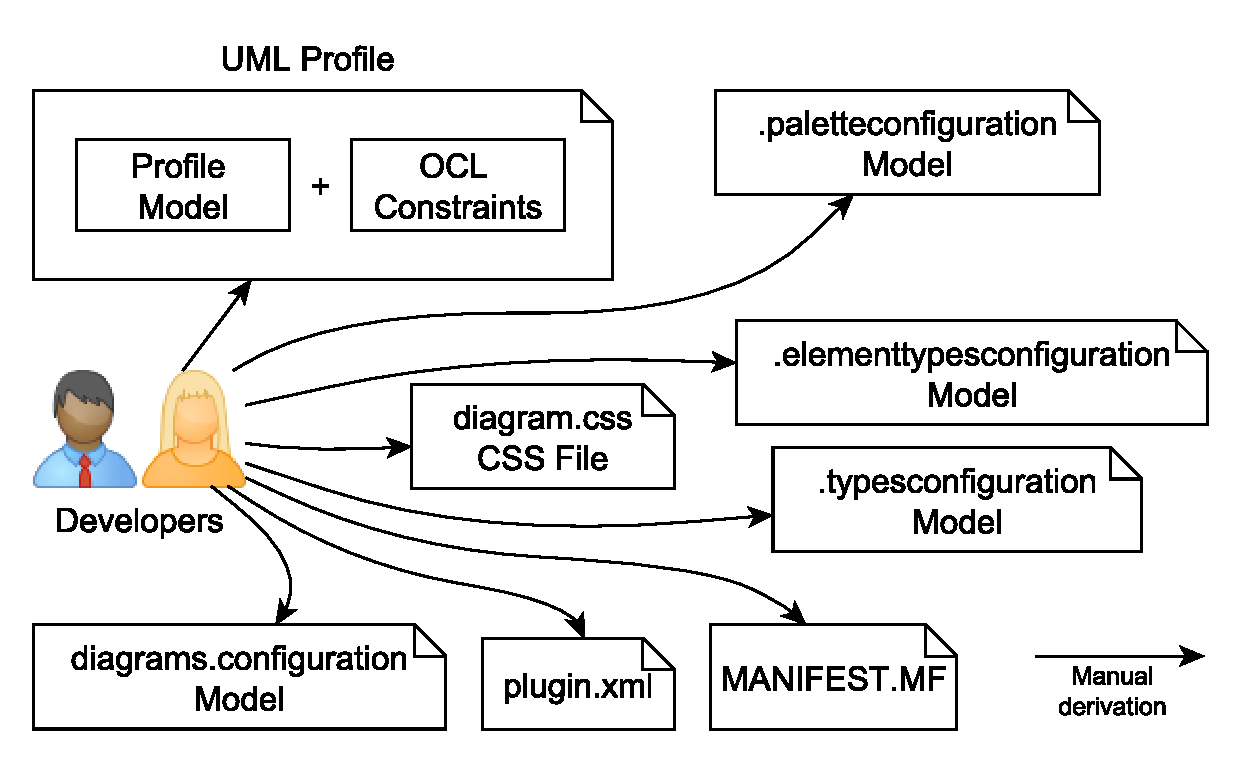
\includegraphics[width=1\textwidth]{diagrams/neededPapyrusFiles.pdf}
	\vspace{-3mm}
	\caption[]{Models/files developers need to write manually to 
		develop a fully functional distributable Papyrus profile editor for Papyrus 2.0.}
	\label{fig:neededPapyrusFiles}
	\vspace*{-3mm}
\end{figure}

The definition of custom shapes for the instantiated \textit{Stereotype}s is another common requirement. 
In Papyrus, Scalable Vector Graphics (SVG) shapes can be bound to \textit{Stereotype}s during the profile creation process. 
However, to make these shapes visible, users need to set the visibility of the shape of \textit{each} \textit{Stereotype} to true. 
Although this is an acceptable trade-off, the users typically need to hide the default shapes by writing custom style rules in a Cascading Style Sheet (CSS), because that by default the SVG shape bound to a \textit{Stereotype} overlaps with the default shape of the base meta-element.
The CSS can be written once but need to be loaded each time \textit{manually} on every diagram that is created. 

To create a distributable graphical editor that has diagrams tailored for the profile and to avoid all the aforementioned drawbacks, users need to create a number of inter-related models and files, and to implement extension points in an Eclipse plug-in project. 
In our previous work \cite{zolotas2018towards} based on Papyrus 2.0, we identified a number of models that need to be created, which is shown in Figure~\ref{fig:neededPapyrusFiles}. 
To create a working UML profile editor in Papyrus, the users typically need to create a Palette Configuration model, an Element Types Configuration model, a Type Configuration model, a Diagram Configuration model, a CSS and Eclipse plug-in related artefact.
However, in our recent studies we discovered that since Papyrus 3.0, the mechanism for creating UML profile editors had changed, altogether with a number of metamodels. 
Figure~\ref{fig:neededPapyrusFiles_new} shows all the artefacts needed to be created for having a distributable Papyrus UML profile editor for Papyrus 3.0+.
In particular, the Palette Configuration metamodel and the Element Types Configuration metamodel (rendered in blue in Figure~\ref{fig:neededPapyrusFiles_new}) had been changed. 
A new metamodel the Architecture metamodel was introduced (rendered in green in Figure~\ref{fig:neededPapyrusFiles_new}). 
To create a UML profile editor, users also need to create a Creation Command Java class to initialise the UML diagram (rendered in green in Figure~\ref{fig:neededPapyrusFiles_new}). 
This introduces addition complications, because the changes were not properly documented, and there is little documentation on how to create models mentioned in Figure~\ref{fig:neededPapyrusFiles_new} in order to create a working UML profile editor.
In addition, it is also a labour-intensive and error-prone process to migrate editors created based on Papyrus 2.0 to Papyrus 3.0+, for the users typically need to create new Palette Configuration and Element Types Configuration models, as well as the new concepts such as the Architecture model.

\begin{figure}[ht!]
	\centering
	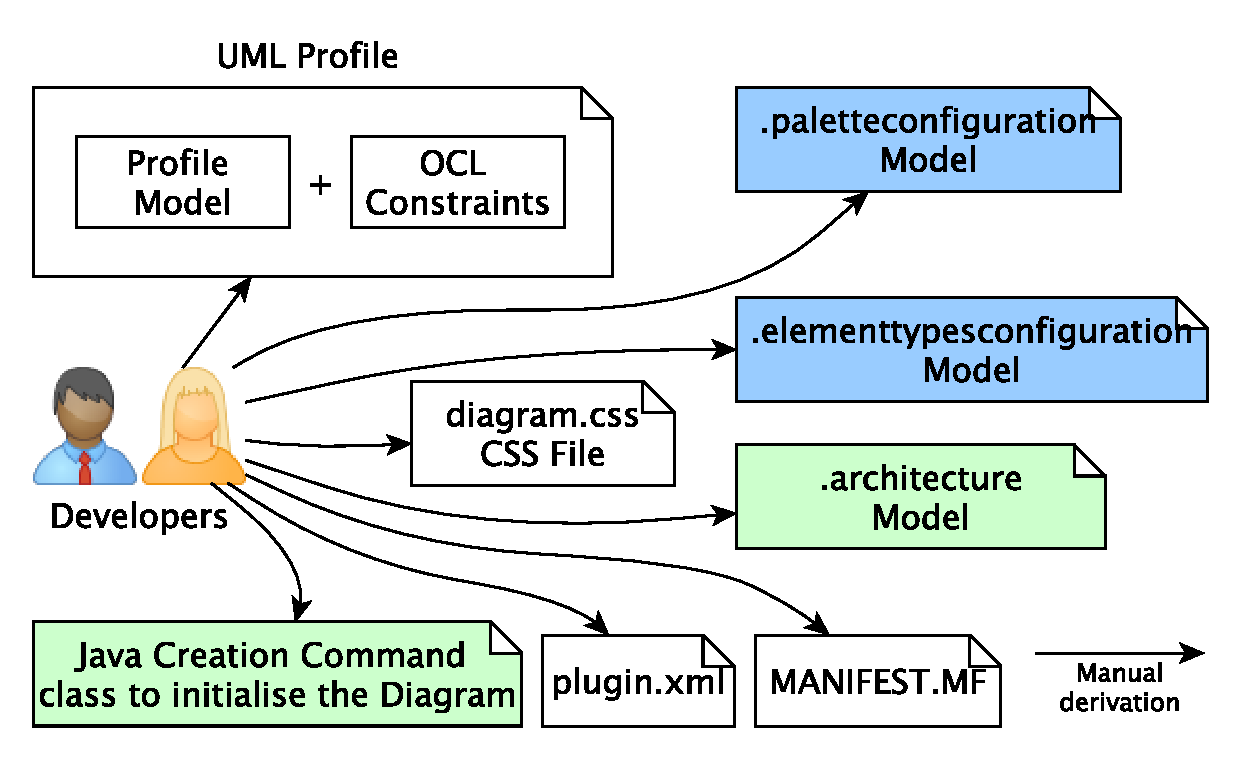
\includegraphics[width=1\textwidth]{diagrams/neededPapyrusFiles_new.pdf}
	\vspace{-3mm}
	\caption[]{Models/files developers need to write manually to 
		develop a fully functional distributable Papyrus profile editor for Papyrus 3.0+.}
	\label{fig:neededPapyrusFiles_new}
	\vspace*{-3mm}
\end{figure}


UML profile editors created using approaches in Figure~\ref{fig:neededPapyrusFiles} and Figure~\ref{fig:neededPapyrusFiles_new} both have custom palette, with which the users are able to create elements in their DSL (UML meta-elements with \textit{Stereotype}s defined in the UML profile applied automatically to them).
Detailed discussions about the artefacts needed in order to create a UML profile editor are provided in Section~\ref{sec:implementation}.
A few hundred lines of code need to be written while tedious Plug-in creation and repetitive model creation tasks should be done. \will{This is not necessarily the case, the claim is too strong}

This \textit{labour-intensive}, \textit{repetitive} and \textit{error-prone} process could be automated. 
In this paper, we present our tool - Jorvik, which uses a single-source input to automatically generate a UML profile and models/files mentioned above for a UML profile editor. 
This approach is described in Section~\ref{sec:approach} that follows. 

\section{Proposed Approach}
\label{sec:approach}

\sg{In order to minimise the labour intensive and repetitive process required for the definition of a UML Profile and its relevant Papyrus-specific implementation level artefacts, we propose Jorvik, an automatic generation tool for Papyrus UML profiles and their editors. }\SG{Identical to the sentence above.} 
Through Jorvik, developers can define the abstract syntax and the concrete (graphical) syntax of their DSLs (the UML profile) in the form of an annotated Ecore metamodel.
The annotations can be used to specify the \textit{Stereotyp}s to be created in the UML profile, and what meta-elements they extend. 
With the annotations, the developers can also specify the graphical syntax and related information (e.g. shapes for the \textit{Stereotype}s and the icons for the creation tools in the palette). 
The annotated Ecore metamodel is then processed by Jorvik and transformed into a UML profile and related Papyrus-specific models/files needed for a standalone Papyrus editor. This is done hrough a series of model management operations like model validation, model-to-model (M2M) and model-to-text (M2T) transformations. An overview of our proposed approach is presented in Figure~\ref{fig:approachOverview}. 
We discuss the steps involved in the process in detail in the remainder of this section, followed by a running example. 
Technical details about the different steps of the proposed approach are provided in Section~\ref{sec:implementation}.

\begin{figure}[ht!]
	\centering
	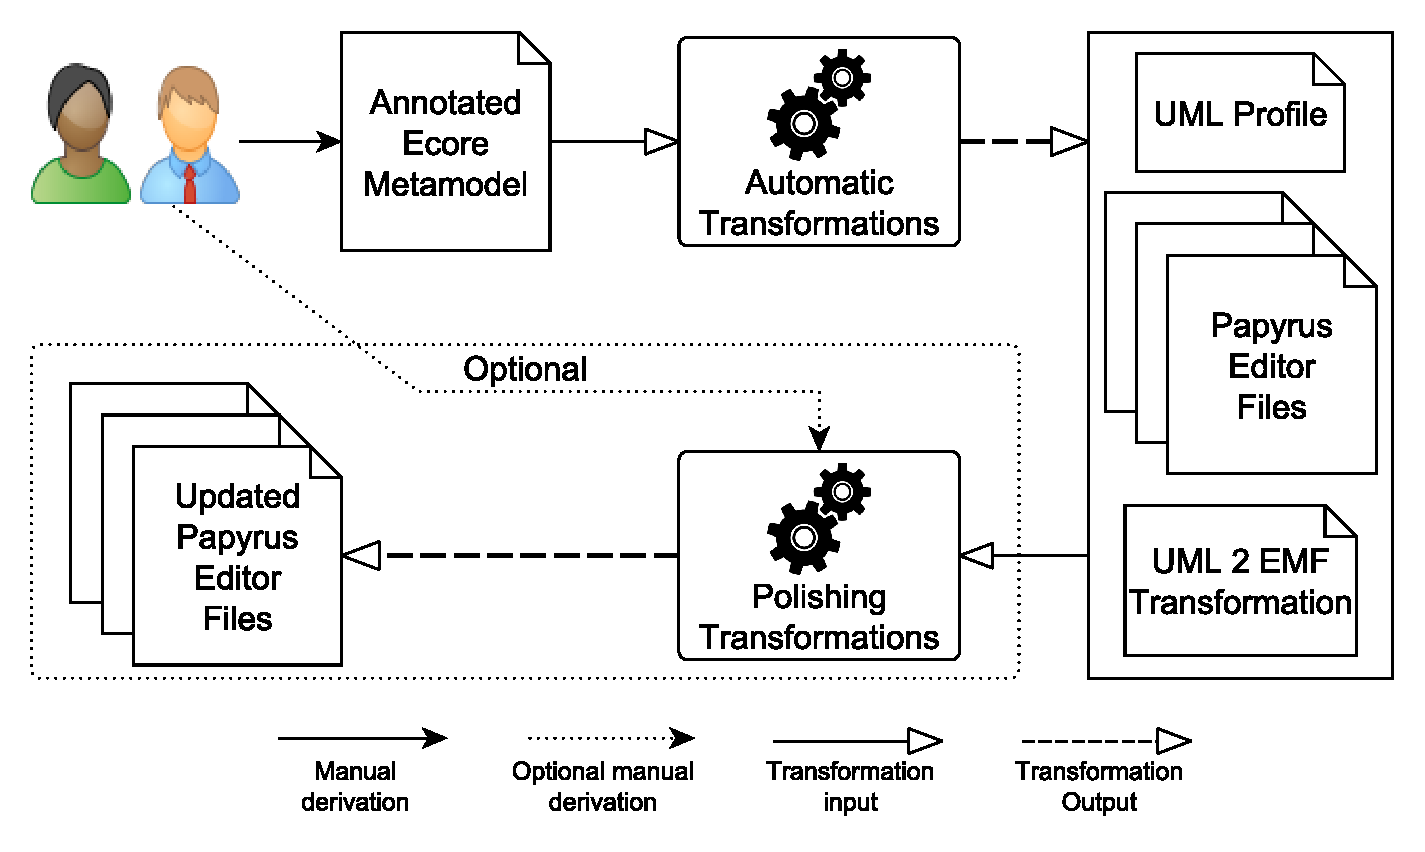
\includegraphics[width=1\textwidth]{diagrams/approachOverview.pdf}
	\caption[]{An overview of the proposed approach}
	\label{fig:approachOverview}
%	\vspace{-6mm}
\end{figure}

The first step is to create an annotated Ecore metamodel to define the intended DSL.
In order to do this, a number of annotation keywords are defined for the users to use:

\begin{enumerate}[label=\arabic*.]
	\item \textbf{@Diagram} annotations are used to define diagram-specific information like the name and the icon of the diagram. This annotation can be applied to EPackages and should always be applied to the EPackage at the top level.
	\item \textbf{@Node} annotations are used to indicate the \textit{Stereotype}s that should be instantiated as nodes in the diagrams. 
	The UML meta-element that this \textit{Stereotype} extends is provided through the \emph{base} property. 
	The SVG shape to be used on the canvas and the icon of the specific element in the palette are specified through the \emph{shape} and \emph{icon} properties, respectively. 
	\item \textbf{@Edge} annotations are used to denote \textit{Stereotype}s that should be instantiated as edges in the diagrams. 
	The UML meta-element extended by this stereotype is provided through the \emph{base} property. The icon of the specific element in the palette is also passed as property along with the desired style of the line. 
	This annotation can be applied either to an EClass or to an EReference.
\end{enumerate}

In the metamodel, all annotated \textit{EClass}es are automatically transformed into \textit{Stereotypes}.
\textit{Stereotype}s are also created from annotated EReferences (more about this below). 
Depending on the required graphical syntax of the \textit{Stereotype} (i.e., if it should be represented as a \textit{node} or as an \textit{edge} on the diagram), developers need to use the appropriate annotation on EClasses/EReferences. 
A detailed list of all valid annotation properties is provided in Appendix~\ref{appendixA}. 

With the annotated Ecore metamodel in place, the next step is to check the validity of the annotations in order to proceed with the generation process. 
Therefore, a custom-made model validation script written in the Epsilon Validation Language (EVL)~\cite{evlKolovos} (see Figure~\ref{fig:approachOverview}) is used.
The validation rules (which we describe in detail in Section~\ref{sec:implementation}) check if the annotations provided and their attributes match the expected ones by Jorvik (e.g., each annotated element includes a reference to the UML base element it extends). 
If the validation fails, feedback is provided to users to fix the problems detected. 
Otherwise, the annotated Ecore metamodels are consumed by a workflow of M2M and M2T  transformations illustrated in Figure~\ref{fig:transformationWorkflow} and described in detail in Section~\ref{sec:implementation}. 
The transformations are written in the Epsilon Transformation Language (ETL)~\cite{Kolovos2008} and the Epsilon Generation Language (EGL)~\cite{rose2008egl}. 
In principle, any other model validation, M2M and M2T language could be used (e.g., ATL~\cite{jouault2006atl}). 
The transformations produce the UML profile with the appropriate OCL constraints and all the configuration models and files needed by Papyrus. 
In addition, an M2M transformation is also generated that can be used later by developers to transform the UML models that conform to the generated UML profile, back to EMF models that conform to the Ecore metamodel used as source. 
Model management programs already developed to run against model conforming to the EMF metamodel can be re-used.

Jorvick offers the option of \textit{polishing transformations}, where developers are able to write their own (optional) transformations to fine-tune the generated artefacts produced by the built-in transformations. 
In the following section, the proposed approach is explained via a running example.

\subsection{Running Example}
\label{sec:example}
In this example we define a DSL - the Simple Development Process Language (SDPL) - in an annotated Ecore metamodel and we generate the corresponding UML profile and Papyrus graphical editor using Jorvik.
We start by defining the abstract syntax of the DSL using  Emfatic\footnote{\url{https://www.eclipse.org/emfatic/}}, a textual notation for Ecore, which is shown in Listing~\ref{lst:annotatedSdplEmfatic} (ignore the annotations at this point). 
A process defined in SDPL consists of \textit{Steps}, \textit{Tools} and \textit{Persons} participating in it. 
Each \textit{Person} is familiar with certain tools and can have different \textit{Role}s in steps of a process, while each step refers to the next step that follows using the \textit{next} reference.

\begin{figure}[t]
	\lstinputlisting[caption={The annotated Emfatic code that defines the 
		metamodel 
		of\\ SDPL and can be used to generate the UML profile and the 
		associated \\Papyrus 
		editor.},
	label={lst:annotatedSdplEmfatic},
	captionpos=b, 
	language=Emfatic, 
	tabsize=2, 
	numbers=left, 
	numbersep=5pt, 
	numberstyle=\tiny,  
	breaklines=true]{sdplAnnotated.emf}
	\vspace*{-5mm}
\end{figure}

In order to generate the UML profile and the Papyrus graphical editor we need to add the following concrete syntax-related annotations shown in Listing~\ref{lst:annotatedSdplEmfatic}:

\begin{itemize}
	\item[--] \textbf{Line 2:} The name and the icon that should be used by Papyrus in the custom diagrams menus are defined using the \textit{name} and \textit{icon} properties of the \textit{@Diagram} annotation.
	\item[--] \textbf{Lines 5, 10 \& 15:} The \textit{@Node} annotation is used to define that the three concepts (i.e., Steps, Roles and Tools) should be \textit{Stereotype}s in the UML profile that will be represented as nodes on the diagram. 
	The \textit{base} parameter is used to define which UML meta-element the \textit{Stereotype} should extend (i.e., \textit{Class}\footnote{Although profiles are meant to accommodate ``natural'' extensions to UML artefacts, sometimes is the case that generic meta-elements are used instead. 
	For example, in the Archimate for Papyrus tool presented in Section~\ref{sec:efficiencyEvaluation}, the Use Case meta-element is used as base for the \textit{Business Service} \textit{Stereotype}, or Class as the base for the \textit{Business Role} \textit{Stereotype}. 
	Thus, the selection of the most appropriate base element is left for the user.} in the \textit{Stereotype}s of this example\footnote{\textit{Class} is actually \textit{UML::Class}, we omit the ``UML::'' prefix to \sg{reduce the efforts for the user???? (Perhaps ``to improve clarity''?)}}). The shape on the canvas and the icon in the palette for each \textit{Stereotype} are given using the \textit{shape} and \textit{icon} annotation details. We also change the font style by setting the bold details to true (see line 10).
	\item[--] \textbf{Line 19 \& 22} The EReference \textit{familiarWith} and the \textit{Role} EClass are added in the profile as \textit{Stereotype}s that extend the meta-element \textit{Association} of UML (UML::Association). 
	These \textit{Stereotype}s should be represented as links in the diagrams and thus are annotated with the \textit{@Edge} string.
	In contrast to the \textit{familiarWith EReference}, the types the 
	\textit{Roles} edge should be able to connect are not know and need to be 
	specified as properties of the annotation (i.e., \textit{source=``src''} 
	and \textit{target=``tar''}). 
	This denotes that the source/target nodes of this connector are mapped to the values of the
	EReferences: \textit{src} and \textit{tar} respectively. We also set the \sg{font size }\SG{font height in the script} to 15 for the labels of the \textit{familiarWith} edges (see line 19).
	\item[--] \textbf{NB Line 8:} The \textit{next} EReference is not required to be displayed as an edge on the diagram thus it is not annotated with \emph{@Edge}. 
	However, it will be a property of the \textit{Step} \textit{Stereotype} in the generated profile, so it can be set in the model (but it will not be displayed on the diagram).
\end{itemize}


The automated M2M and M2T transformations discussed above are then executed on the Ecore file and the produced SDPL Papyrus editor is presented in Figure~\ref{fig:sdplEditor}.  \thanos{The figure should be updated to include the bold label for Tool and the 15 font for familiarWith.}

\begin{figure}[ht!]
	\centering
	\includegraphics[width=1\textwidth]{images/sdplEditor.png}
	\caption[]{The SDPL editor for Papyrus where two steps in the software 
		development process are defined and responsible persons are attached to 
		them\\ along with the tools they are specialized on.}
	\label{fig:sdplEditor}
\end{figure}

\subsection{Polishing Transformations}
The generated editor is fully functional but it can be further customised to fit users' custom needs. 
For example, by default, our automatic transformations dictate the diagram, through the CSS file to show the stereotype name applied to each node. 
However, in this example we want to hide the stereotype names and display labels in red font. 
This can be achieved by manually amending the generated CSS file. 
However, the CSS file will be automatically overridden if the user regenerates the profile and the editor in the future (e.g., because of a change in the metamodel). 
To avoid this, the user can use the -- optional -- CSS generation polishing transformation (\#5b in Figure~\ref{fig:transformationWorkflow}) shown in Listing~\ref{lst:cssPolishingExample}. 
Every time the profile and editor generation is executed, the polishing transformation will be called and will set the visibility of the stereotypes to false automatically. 

\begin{figure}
	\lstinputlisting[
	caption={The polishing transformation for the CSS file generation that\\ sets the visibility of the names of the nodes to true.},
	label={lst:cssPolishingExample},
	captionpos=b, 
	language=EGL, 
	tabsize=2, 
	numbers=left, 
	numbersep=5pt, 
	numberstyle=\tiny, 
	breaklines=true]
	{cssPolishingExample.egl}
%	\vspace*{-6mm}
\end{figure}

%\dk{What about inheritance? If a class is annotated as @Node and its 
%subclasses are annotation-less do they inherit the @Node annotation and its 
%details?} Thanos: No...

The EGL template in Listing~\ref{lst:cssPolishingExample} generates a CSS rule in lines 1-3 that sets the visibility property of the stereotypes' labels to false. 
It stores all the elements in the Ecore metamodel that are annotated as @Node (line 6) in a collection and iterates though them in lines 7-10. 
For each of the node stereotypes, it generates the static text ``[appliedStereotypes~='' followed by the name of each stereotype and a comma. 
At the end it prints the curly brackets (lines 10 and 12) and the text ``fontColor:red;'' in line 11. 
The resulted output that is amended automatically in the original CSS file by the polishing transformation is the one shown in Listing~\ref{lst:cssPolishingOutput}.

\begin{figure}[ht!]
	\vspace*{-5mm}
	\lstinputlisting[caption={The output that is amended in the original CSS 
		file using the\\ CSS polishing transformation of 
		Listing~\ref{lst:cssPolishingExample}},label={lst:cssPolishingOutput},captionpos=b,
	language=CSS, tabsize=2, numbers=left, numbersep=5pt, numberstyle=\tiny, 
	breaklines=true]{cssPolishingOutput.egl}
%	\vspace*{-5mm}
\end{figure}

%Beyond providing a disciplined mechanism for customising the produced UML 
%profile and editor polishing transformations also offer an extension point for 
%future evolution of the proposed approach: user defined polishing 
%transformations developed to fulfil scenarios that we do support can be created 
%and submitted to be included in the default transformations of our approach.
%\sg{This paragraph is unclear}.


\section{Implementation}
\label{sec:implementation}
In this section, we discuss the technical implementation of Jorvik which underpins the process of our approach discussed in the previous section. 

Figure~\ref{fig:transformationWorkflow} shows the transformations workflow. 
Each transformation is identified by a number (\#2-\#8 in Figure~\ref{fig:transformationWorkflow}) for easier reference. 
In addition to the transformations, a pre-transformation validation script (\#1 in Figure~\ref{fig:transformationWorkflow}) is executed to verify the correctness of the annotations and provide useful feedback to the users if there is anything wrong. 
Moreover, supporting files needed for the creation of the Papyrus plugin are also generated while icons and shapes are placed next to the annotated metamodel (\#8 in Figure~\ref{fig:transformationWorkflow}). 
As the transformations consists of about 1000 lines of code we will describe them omitting low level technical details\footnote{Full implementations and instructions are available at \url{https://github.com/wrwei/Jorvik}}. 

\begin{figure}[ht!]
	\centering
	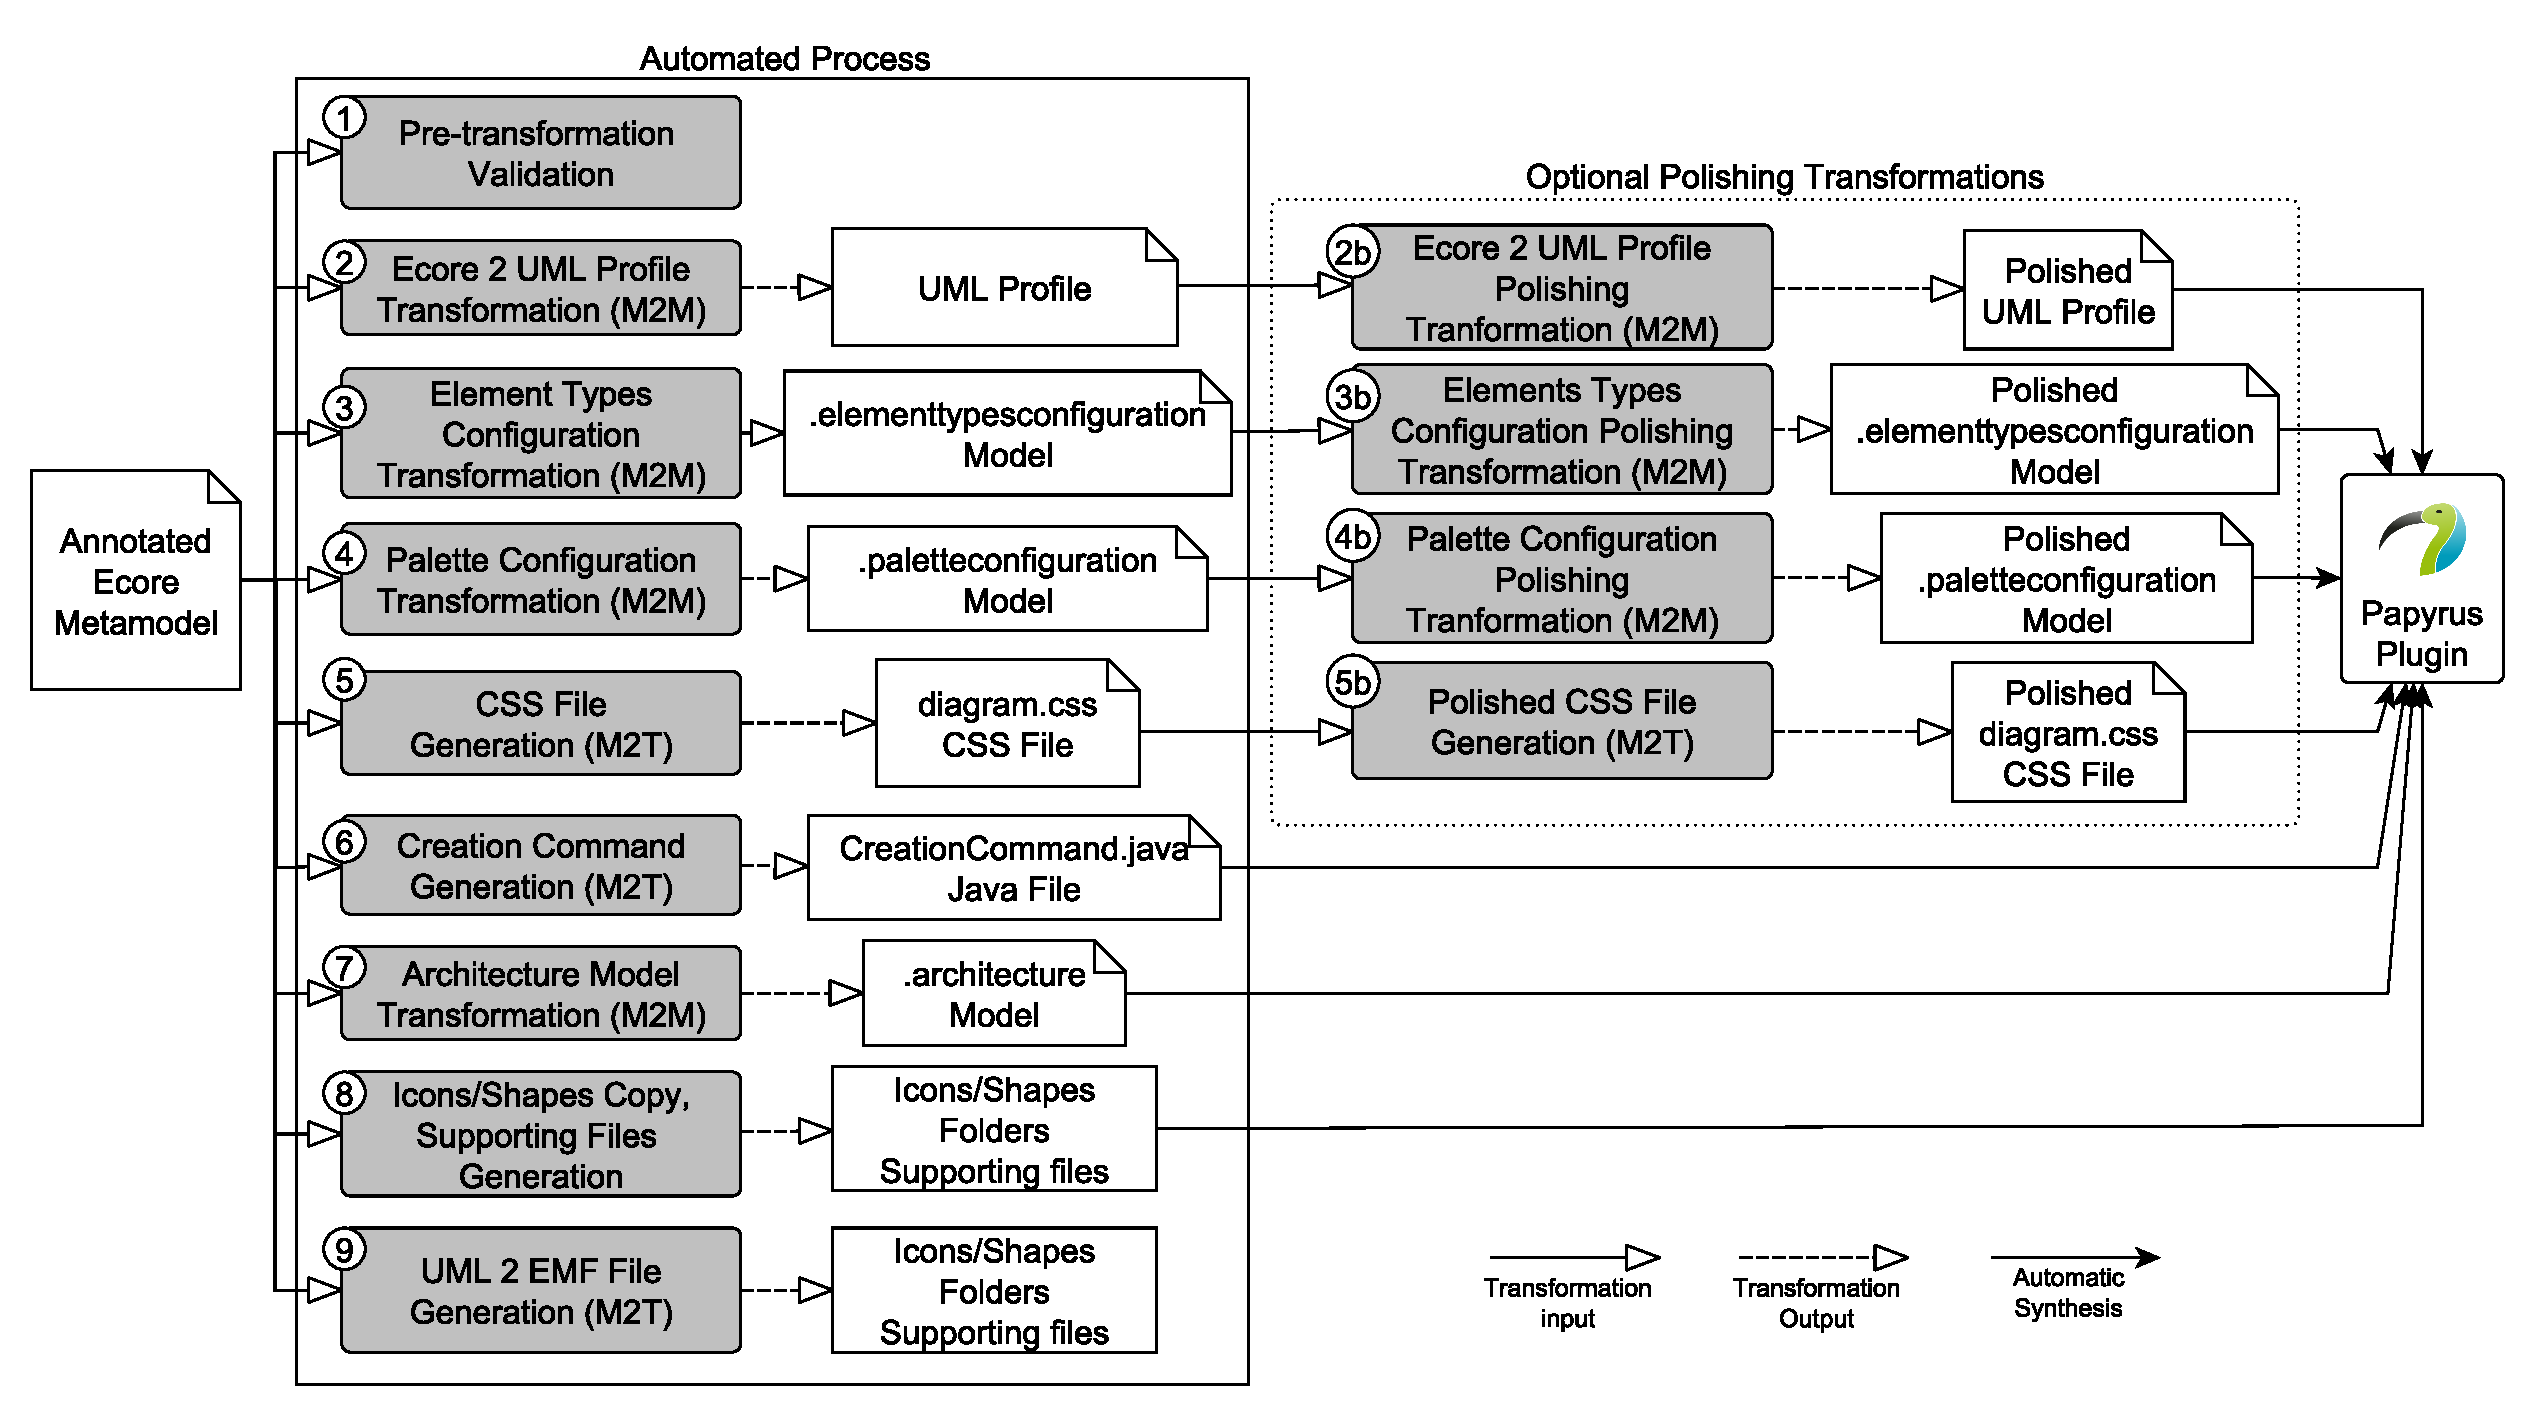
\includegraphics[width=1\textwidth]{diagrams/transformationWorkflow.pdf}
	\caption[]{An overview of the transformation workflow}
	\label{fig:transformationWorkflow}
%	\vspace*{-3mm}
\end{figure}

\subsection{Pre-transformation Validation (\#1)}
To check the correctness of the annotated ECore metamodel, a model validation program is firstly executed against the metamodel.
The program is written using EVL and consists of several rules that check if the annotated ECore elements have all the necessary information (e.g., a UML base class) and if the values provided are correct (e.g., font size for labels is a positive integer). 
Listing~\ref{lst:evlRulesBold} presents an example of a rule written in EVL which checks if the value provided for the ``bold'' details in a @Node annotation is correct (i.e., true or false). More specifically, in lines 2--3 a guard is applied to check that the rule is only applied to elements that have the @Node annotation attached to them (line 2) while tests the rule only on those annotations that have the ``bold'' detail defined (line 3). 
In lines 4--6, the condition to check is provided, which is that the value of the ``bold'' detail is either \textit{true} or \textit{false}. 
Finally, in line 7--8 a message is displayed to the users in case the rule is violated providing information regarding the acceptable values and the name of the element(s) that violated this rule.

\lstinputlisting[
caption={Example a rule that check that the values provided to the ``bold'' styling detail for @Node annotations is correct.},
label={lst:evlRulesBold},
captionpos=b, 
language=EVL, 
tabsize=2, 
numbers=left, 
numbersep=5pt, 
numberstyle=\tiny, 
breaklines=6true]{evlRulesBold.evl}

\begin{table}[ht!]
	\begin{tabular}{|l|L{5cm}|L{5cm}|}
		\hline
		\textbf{\#} & \textbf{Rule Description} & \textbf{Condition Checked} \\ \hline
		1 & There is exactly one Diagram annotation & The number of the Diagram annotations is 1 \\ \hline
		2 & Diagram annotation has a name detail & The name detail is defined \\ \hline
		3 & Diagram annotation has acceptable details provided & There are no other details provided rather than name and/or icon \\ \hline
		4 & Node/Edge annotations have base class set & Any string is provided\\ \hline
		5 & Edge annotations of EClasses have source/target defined & The source/target details are defined \\ \hline
		6 & An acceptable lineStyle value for Edge annotations is provided & The value is dashed, solid, dotted, hidden or double\\ \hline
		7 & An acceptable bold value for Node/Edge annotations is provided & The value is either true or false\\ \hline
		8 & An acceptable fontHeight value for Node/Edge annotations is provided & The value is a positive integer\\ \hline
		9 & Node annotations have acceptable details provided & There are no other details provided rather than base, fontHeight and/or bold \\ \hline
		10 & Edge annotations have acceptable details provided & There are no other details provided rather than base, source, target, fontHeight, bold, and/or lineStyle\\ \hline
	\end{tabular}
	\caption{The list of the rules checked for the annotated ECore metamodel.}
	\label{tab:evlRules}
\end{table}

Table~\ref{tab:evlRules} enumerates all the rules applied along with their descriptions and the conditions to be checked. 
The implementation of the rules in EVL can be found in the paper's webpage\footnote{\url{https://github.com/wrwei/Jorvik}}. 


\subsection{EMF to UML Profile Generation (\#2)}
\label{sec:profileGeneration}
The EMF to UML Profile Generation executes a Model-to-Model transformation written in ETL. 
The source model of this transformation is the annotated Ecore metamodel (e.g,  Listing~\ref{lst:annotatedSdplEmfatic}) and the target model is a UML profile model.
This transformation consists of two main rules, one that creates a \textit{Stereotype} for each EClass element of the metamodel and a second that creates a \textit{Stereotype} for each EReference annotated as @Edge.

\begin{itemize}
	\item[--] \textbf{rule eclass2stereotype:} This transformation rule transforms each EClass element in the annotated Ecore metamodel to an element of type \textit{Stereotype} in the target UML model. 
	All attributes of each EClass are also transformed across to the created \textit{Stereotype}. 
	\item[--] \textbf{rule reference2stereotype:} This rule creates a new \textit{Stereotype} with the same name in the UML profile model for each of the \textit{EReferences} that are annotated as @Edge in the Ecore metamodel. 
	No attributes are added to the stereotype as EReferences do not support attributes in Ecore\footnote{It is the users' responsibilities to make sure that they handle name collisions for EReferences themselves (for that EClasses may have EReferences with the same name).}.
\end{itemize}

When all stereotypes are created, a number of post-transformation operations are executed to 1) create the generalisation relationships between the \textit{Stereotype}s, 2) add the references/containment relationships between the \textit{Stereotype}s, 3) create the extension with the UML base meta-element and 4) generate and add the needed OCL constraints for each edge: 

\begin{enumerate}[label=\arabic*)]
	\item For each of the superclasses of an EClass in the metamodel we create a \textit{Generalisation} UML element. 
	The generalisation element is added to the stereotype created for this specific EClass and refers via the \textit{generalization} reference to the stereotype that was created for the superclass.
	\item For each reference (ref or val) in the metamodel a new \textit{Property} UML element is created and added to the \textit{Stereotype} that represents the EClass. 
	A new \textit{Association} UML element should also be created and added to the \textit{Stereotype}. The name and the multiplicities are also set.
	\item By default the \textit{Stereotype}s extend the \textit{Class} base element unless a different value is passed in the \textit{base} property of the @Node/@Edge annotation. 
	In this post-transformation operation the necessary \textit{Import Metaclass} element and \textit{Extension} reference are created and attached to the \textit{Stereotype}.
	\item In the last operation, the OCL constraints are created for each stereotype that will be represented as an edge on the diagram. 
	Two \textit{Constraint} and two \textit{OpaqueExpression} elements are created for each edge \textit{Stereotype} that check the two necessary constraints. 
	The OCL constraints are explained in details in the section that follows.
\end{enumerate}

\subsection{OCL Constraints}
\label{sec:constraints}

To illustrate the OCL constraints, we provide a partial view of the SDPL UML profile in Figure \ref{fig:sample_profile}\footnote{The attributes of the stereotypes are omitted for simplicity.}.

\begin{figure}[ht!]
	\centering
	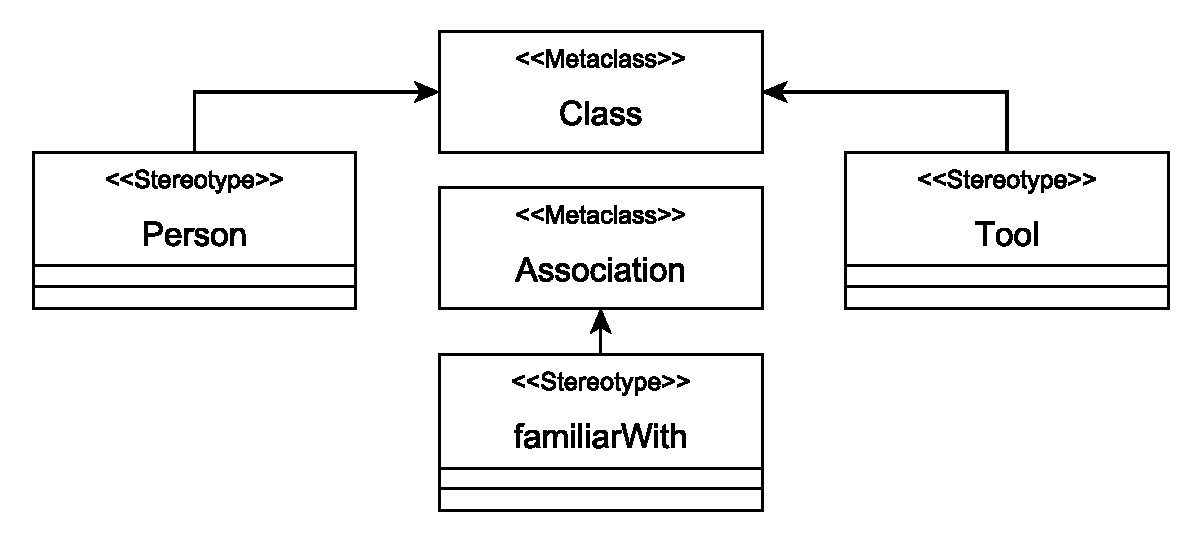
\includegraphics[width=1\textwidth]{diagrams/example_profile}
	\caption[]{Example UML profile for SDPL showing Person, Tool and the familiarWith association}
	\label{fig:sample_profile}
\end{figure}

In Figure \ref{fig:sample_profile}, there are three \emph{Stereotype}s - \emph{Person} and \emph{Tool} both extend meta-element \emph{UML::Class}, and they correspond to classes \emph{Person} and \emph{Tool} in the Emfatic code in Listing \ref{lst:annotatedSdplEmfatic}. 
\emph{Stereotype} \emph{familiarWith}, which extends meta-element \emph{UML::Association}, corresponds to the reference \emph{familiarWith} in the \emph{Person} class in Listing \ref{lst:annotatedSdplEmfatic}.

In Figure~\ref{fig:sdplEditor}, the \textit{familiarWith} association is used to connect \textit{Person} \emph{Alice} with \textit{Tool} \emph{StarUML}. 
However, the \emph{familiarWith} stereotype can be applied to any \emph{Association}, and not strictly to \emph{Associations} which connect \emph{Person} and \emph{Tool} stereotyped elements. 
Therefore, constraints are needed to check (at least) two aspects:

\begin{itemize}
	\item \textbf{End Types}: the elements that a \emph{familiarWith} association connects to that have \emph{Person} and \emph{Tool} \textit{Stereotype}s applied to them;
	\item \textbf{Navigability}: the \emph{familiarWith} association starts from an element stereotyped as \emph{Person} and points to an element stereotyped as \emph{Tool}.
\end{itemize}

\subsubsection{End Types}
Listing \ref{lst:endTypes} shows the OCL code for the \emph{End Types} constraint. 
Line 1 accesses the types that \emph{familiarWith} connects. 
Lines 3 and 4 check if the types that \emph{familiarWith} connects are of type that either has \textit{Stereotype} \emph{Person} or \emph{Tool}. 
In this way, if a \emph{familiarWith} association connects two types that are not \emph{Person} or \emph{Tool}, the constraint fails.

\lstinputlisting[
	caption={The End Types constraint in OCL},
	label={lst:endTypes}, 
	captionpos=b, 
	language=OCL, 
	tabsize=2, 
	numbers=left, 
	numbersep=5pt, 
	numberstyle=\tiny, 
	breaklines=true, 
	escapeinside={(*}{*)}]{endtypes.txt}

\subsubsection{Navigability}
Listing \ref{lst:navigability} shows the OCL code for the \emph{Navigability} constraint. 
In this case, we are interested in checking the \emph{isNavigable} property of each end. 
Thus, in lines 2 and 3, we obtain the member ends that \emph{familiarWith} connects with. 
If these ends are obtained successfully (line 4), we check that the \emph{personEnd} (connecting element stereotyped as \emph{Person}) is not navigable (line 5) and the \emph{toolEnd} (connecting element stereotyped as \emph{Tool}) is navigable (line 6). 
Therefore, we are checking that a \emph{familiarWith} association can only go from \emph{Person} to \emph{Tool} and not the other way around. 
We need to highlight, that currently, opposite references are not supported; plans for future work are outlined in Section~\ref{sec:future}.

\begin{figure}[h]
	\lstinputlisting[caption={The Navigability constraint in 
		OCL},label={lst:navigability}, captionpos=b, language=OCL, tabsize=2, 
	numbers=left, numbersep=5pt, numberstyle=\tiny, breaklines=true, 
	escapeinside={(*}{*)}]{navigability.txt}
%	\vspace*{-5mm}
\end{figure}

With these two constraints implemented, we are able to automatically generate OCL constraints for \textit{Stereotype}s that extend \emph{UML::Association}. 
We use the \emph{End Types} and \emph{Navigability} constraints as templates with dynamic sections (where the specific \textit{Stereotype} names are inserted dynamically, e.g., \emph{Person} and \emph{Tool}). 
So far we have only explored constraints for \textit{Stereotype}s that extend \emph{UML::Association}. 
The constraint templates for \textit{Stereotype}s that extend other UML relationships need to be developed separately as the means to access source/target elements of the relationship are different.

\subsection{Element Types Configuration Configuration Transformation(\#3)}
\label{sec:elementTypes}
Apart from the UML profile, Papyrus graphical editor requires an Element Types Configuration model, which associates the \textit{Stereotype}s defined in the UML profile with their abstract syntax (the meta-elements in UML they extend) and their concrete syntax (the graphical notations of the meta-elements in UML they extend). 

This transformation is responsible for creating an Element Types Configuration model (of extension .elementtypesconfiguration) that contains type specialisation information for the \textit{Stereotype}s in the UML profile. 
Since our previous work \cite{zolotas2018towards}, the \textit{ElementTypesConfiguration} metamodel for Papyrus has changed. 
As a result, we have to re-implement this transformation. 
For each \textit{Stereotype}, two \textit{SpecializationTypeConfiguration}s are created, one links the \textit{Stereotype} to its UML meta-element, another links the \textit{Stereotype} to the concrete syntax of its UML meta-element.
For example, a \textit{Stereotype} that extends UML::Class needs to specialise the UML::Class \textit{MetamodelTypeConfiguration}; and it needs to specialise the Class Shape \textit{SpecializationTypeConfiguration} defined in the UMLDI Element Types Configuration model. 
In addition to \textit{SpecializationTypeConfiguration}s, for each \textit{Stereotype} an \textit{ApplyStereotypeAdviceConfiguration} needs to be created, which associates the \textit{SpecializationTypeConfiguration} to the actual \textit{Stereotype} in the UML profile.

The transformed Element Types Configuration model is a crucial part to Papyrus graphical editor creation, it is used in conjunction with other models/artefacts and it drives the creation of model elements in the editor.

\subsection{Palette Configuration Transformation (\#4)}
\label{sec:paletteGeneration}
This transformation is responsible for creating a Palette Configuration model (of extension .paletteconfiguration) that configures the contents of the custom palette for the diagram in Papyrus. 
The model conforms to the \textit{PaletteConfiguration} metamodel that ships with Papyrus, which also changed since our previous work. 
The transformation creates a new \textit{PaletteConfiguration} element and adds two new \textit{DrawerConfiguration} elements that represent the two different tool compartments in our palette (i.e., one for the tools that create nodes and one for those creating edges). 
For each element in the Ecore metamodel annotated as @Node/@Edge a new \textit{ToolConfiguration} element is created and added to the nodes/edges drawer respectively. 
The kind of \textit{ToolConfiguration} are decided based on the @Node/@Edge annotation, for nodes, the kind is \textit{CreationTool}, for edges, the kind is \textit{ConnectionTool}.
An \textit{IconDescriptor} element is also created and added to the \textit{ToolConfiguration} pointing to the path of the icon for that tool (this is the path passed as argument to the \textit{icon} property of the @Node/@Edge annotation).
Finally, for each \textit{ToolConfiguration}, they need to refer to the element types they conform to, which are defined in the Element Types Configuration model transformed in Step \#3. 
In this way, when an element is created in the diagram using the palette, behind the scene, Papyrus is able to locate the \textit{Stereotype} and infer the UML syntax they specialise.

\subsection{CSS File Generation (\#5)}
\label{sec:cssGeneration}
As stated above, in Papyrus, the look and feel of diagram elements can be customised using CSS. 
In this transformation we generate the CSS style rules that define the appearance of nodes and edges in diagrams. 
Each node on a diagram has a set of compartments where the attributes, the shape, etc. appear. 
Initially, for all nodes that will appear on the diagram, we create a CSS rule to hide all their compartments and another rule to enable the compartment that holds the shape. 
The latter rule also hides the default shape inherited from the meta-element tat the stereotype extends. 
Then, for each stereotype that appears as a node, a CSS rule is generated to place the SVG figure in the shape compartment. 
For elements of type \textit{Stereotype}, the connection of the SVG figure to the stereotypes is achieved by assigning the path of the SVG file to the \textit{svgFile} property available in CSS. 
Finally, we generate the CSS rules for each edge, e.g., if a \emph{lineStyle} parameter is set, then the \textit{style} property for that Edge stereotype is set to the value of the lineStyle parameter (e.g., ``solid'', ``dashed'', etc.).

\subsection{Creation Command Generation (\#6)}
\label{sec:creationCommand}
In order for Papyrus to create a diagram, it requires the initialisation of the diagram.
The Creation Command is a Java class which is responsible for initialising Papyrus diagrams. 
The Creation Command class is needed since Papyrus 3.0+ (after our previous work).
The rationale for the creation command is that it creates a UML model from the UMLFactory as the root element of the diagram.
The minimal requirement for diagram initialisations are:
\begin{itemize}
	\item UML primitive types: the primitive types need to be imported to the diagram in order for the users to reference to them;
	\item UML profiles: the standard UML profile and the user defined UML profile need to be applied in order to initialise the diagram.
\end{itemize}

In order to apply the user defined UML profiles, they need to use the pathmap defined in their plug-ins, which is explained in \#8.
The Java class is generated using a Model-to-Text transformation written in EGL, with the source model the annotated Ecore metamodel and the output text the CreationCommand.java class.

\subsection{Architecture Model Generation (\#7)}
\label{sec:architectureModel}
Papyrus adopted the notion of an Architecture model in order to describe the architecture of the graphical editors since Papyrus 3.0+.
This transformation syntheses an Architecture model using a model creation program using the Epsilon Object Language (EOL) \cite{kolovos2006epsilon}. 
The program needs 1) the annotated Ecore metamodel for the DSL, 2) the Element Types Configuration model, 3) the Palette Configuration model, 4) the UML metamodel, 5) the Creation Command Java class and 6) the CSS custom style sheet as inputs. 
In particular, in the Architecture model, the generation program creates:
\begin{itemize}
	\item An \textit{ArchitectureDomain} which represents the domain of the DSL;
	\item A number of \textit{Concern}s to describe the concerns of the domain;
	\item A number of \textit{Stekaholder}s involved in the domain;
	\item An \textit{ArchitectureDescriptionLanguage} to describe the architecture, which consists of a number of \textit{Viewpoint}s, a number of \textit{PapyrusDiagram}s. 
	The Element Types Configuration and the Creation Command class are needed in the \textit{ArchitectureDescriptionLanguage}. 
	The Palette Configuration model and the CSS sheets are needed in \textit{PapyrusDiagram}s.
\end{itemize}

The Architecture model then needs to be registered and acts as the entry point to all the models/files for a Papyrus editor, which is done in Step \#9.

\subsection{Icons, Shapes and Supporting Files (\#8)}
\label{sec:supportingFiles}
The approach supports the generation of the UML profile and the infrastructure for the Papyrus diagram in either a new Eclipse Plug-in project or in the same Plug-in project where the annotated Ecore metamodel resides. 
In both scenarios, the ``MANIFEST.MF'', the ``build.properties'' and the ``plugin.xml'' files are created (or overridden respectively). 
%The first includes the list of all the required bundles while the second points the project to the locations of the ``MANIFEST.MF'' and ``plugin.xml'' files. 
The ``MANIFEST.MF'' file includes a list of all required bundles/Plug-ins.
The ``build .properties'' file guides the build process of the Eclipse Plug-in.
The ``plugin.xml'' file includes all the necessary extensions for Papyrus to be able to register the UML profile and create the diagrams (e.g., extensions that point to the Architecture model). 
For the creation of a Papyrus editor, in the ``plugin.xml'', three extension points need to be implemented:
\begin{itemize}
	\item \textit{org.eclipse.emf.ecore.uri\_mapping}, in which the users create a mapping between the path of the folder that hold their UML profile, and a PATHMAP, which they can reference in the files/models they create;
	\item \textit{org.eclipse.papyrus.uml.extensionpoints.UMLProfile}, which points to the location of the UML profile that the users define;
	\item \textit{org.eclipse.papyrus.infra.architecture.models}, which points to the location of the Architecture model that the users define in Step \#7.
\end{itemize}

For the scenario where the Papyrus Plug-in is created as a new project, the shapes (SVG files) and the icons (PNG files) are copied to the newly created Plug-in project. 
For the scenario where the UML profile and editor is generated in the same project in which the Ecore source file resides, the shapes and icons files do not need to be copied as they already exist.

Finally, two files that only consist of the XML and the XMI header (namely ``*.profile.di'' and ``*.profile.notation'') are generated. 
These files are necessary for Papyrus to construct the UML profile model\footnote{The diagram layout information requires coordinates related information in the diagram, therefore it is not related to this work}. 

\subsection{UML to EMF Transformation Generation (\#9)}
\label{sec:uml2emf}
This M2T transformation generates the ETL file that can be used to transform the UML models created in Papyrus and conform to the UML Profile generated by our approach, back to EMF models that conform to the source Ecore metamodel given as input to the approach. 
One rule is generated for each of the stereotypes that transforms them back to the appropriate type of the Ecore metamodel. 
Each stereotype has the same attributes and references as the original EClass, therefore, this EGL script also generates the statements in each rule that populate the attributes and the references of the newly created instance of each EClass with the equivalent values of the UML model. 
An example of an auto-generated rule is shown in Listing~\ref{lst:etlGeneratedRule}. 
This rule transforms elements stereotyped as ``Person'' in the UML model to elements of type ``Person'' in an EMF model which conforms to the Ecore metamodel presented in Listing~\ref{lst:annotatedSdplEmfatic}.

\lstinputlisting[
caption={Example of an auto-generated ETL rule that transforms \\elements stereotyped as ``Person'' in the UML model to elements of \\type ``Person'' in an EMF model.},
label={lst:etlGeneratedRule},
captionpos=b, 
language=ETL, 
tabsize=2, 
numbers=left, 
numbersep=5pt, 
numberstyle=\tiny, 
breaklines=true]{etlExample.etl}

%Epsilon Transformation Language (ETL) \cite{} is a hybrid model-to-model transformation languages which provides both a declarative rule-based execution scheme and imperative features for handling complex transformation scenarios. In Listing~\ref{lst:etlGeneratedRule}, rule \emph{PersonUML2PersonEMF} is responsible to transform a \emph{Person} in the UML model to a \emph{Person} in the EMF model. 

ETL provides the $::=$ operator for rule resolution. 
The ETL engine keeps transformation traces which links source elements to target elements of the transformation. 
When $::=$ is used, the ETL execution engine inspects the established transformation traces and invokes the applicable rules (if necessary) to calculate the counterparts of the source elements contained in the collection. 

%If \emph{equivalents()} is applied to a single element, it returns a collection which contains the counterpart(s) of the element in the target model. If \emph{equivalents()} is applied to a collection of elements, it returns a collection of collection (each collection in the result contains the counterparts of the element in the target model). 

In our example (line 6 in Listing \ref{lst:etlGeneratedRule}), the expression ``s.familiarWith'' returns a collection of \emph{UMLProcess!Tool}s (denoted by $ct$). By using ``::='', the ETL engine will look for the rules that transform \emph{UMLProcess!Tool} to \emph{EMFProcess!Tool} and invoke the rules if 
necessary (if the source elements have not been transformed, as shown in the transformation trace) and put the transformed elements into sub-collections 
(denoted by $sc$). 
After the ETL engine goes through all the elements in $ct$, the sub-collections $sc$s are returned (flattened to a single collection if more than one) and are added to ``t.familiarWith''.



\subsection{Polishing Transformations (\#1b - \#6b)}
\label{sec:transformationPatches}
For transformations \#1 - \#6, users are able to define polishing transformations that complement those included in our implementation. 
After each built-in transformation is executed, the workflow looks to find a transformation with the same file name next to the Ecore metamodel. 
If a file with the same name exists, it is executed against the Ecore metamodel and targets the already created output model of the original transformation. 
The execution of the polishing transformation is set \textit{not} to overwrite the target model but to refine it instead.
Table~\ref{tab:polishingTransformationsNames} shows the names that each polishing transformation is expected to have.

\begin{table}[h]
	\caption{Polishing Transformations File Names}
	\centering
	\setlength{\tabcolsep}{3.5pt} 
	\begin{tabular}{|c|c|}
		\cline{1-2}
		\textbf{Transformation ID}  & \textbf{Required File Name}\\ \hline
		\textbf{\#2} & emf2umlProfile.etl\\ \hline
		\textbf{\#3} & elementTypesConfigurationsM2M.etl\\ \hline
		\textbf{\#4} & paletteConfigurationM2M.etl\\ \hline
		\textbf{\#5} & cssFileGeneration.egl\\ \hline
		\cline{1-2}
	\end{tabular}
	\label{tab:polishingTransformationsNames}
\end{table}

\section{Evaluation}
\label{sec:evaluation}

In this section we evaluate AMIGO in two different ways. 
Firstly, we apply it to generate a Papyrus editor for the non-trivial Archimate 
UML profile~\cite{iacob2009archimate,haren2012archimate}. The Adocus Archimate 
for Papyrus\footnote{\url{https://github.com/Adocus/ArchiMate-for-Papyrus}} is 
an open-source tool that includes a profile for Archimate and the appropriate 
editors for Papyrus. This way, we can compare the proportion of the tool that 
AMIGO is able to generate automatically, check the number of polishing 
transformations that the user needs to write to complete the missing parts and 
finally, identify the aspects of the editor that our approach is not able to 
generate. As a result we can to measure the \textit{efficiency} of AMIGO in generating profiles/editors against an existing relatively large 
profile/editor. 

Secondly, we assess the completeness of our approach by applying it on a number 
of other metamodels collected as part of the work presented 
in~\cite{williams2013metamodels}. This way, the approach is tested to check if 
it can successfully generate profiles and editors for a wide variety of 
scenarios.

\subsection{Efficiency}
\label{sec:efficiencyEvaluation}
The Archimate for Papyrus tool offers five kind of diagrams (i.e., Application, Business, Implementation and Migration, Motivation and Technology diagrams). Each of the diagrams uses different stereotypes from the Archimate profile. 

As shown in Figure~\ref{fig:approachOverview}, our approach starts by 
implementing the Ecore metamodel for the profile/editor we would like to 
generate. Thus, in this scenario we need to create the 5 Ecore metamodels and 
annotate those EClasses/EReferences that need to appear as nodes or edges on 
the diagrams. The profiles for each type of Archimate diagram and the editors 
can now be generated. At this point, five fully functional editors are 
generated that can be used to create each of the five types of diagrams that 
the Archimate for Papyrus tool also supports. 

Nevertheless, our generated editors do 
not offer some special features that the Archimate for Papyrus tool offers. For 
example, the latter offers a third drawer in the palette for some diagrams that 
is called ``Common'' and includes two tools (i.e., ``Grouping'' and 
``Comment''). Another feature that is not supported by our default 
transformations is the fact that in Archimate for Papyrus, users are able to 
have the elements represented either by their shapes or by a coloured rectangle 
depending on the CSS class applied to them. In order to be able to implement 
such missing features, we need to write the extra polishing transformations. 
For brevity, we will not go into details on the content of the polishing 
transformations for this specific example.

Table~\ref{tab:evaluation}, summarises the lines of code we had to write manually to generate each file needed by Papyrus to create the 5 basic diagrams (column ``AMIGO'' / ``Handwritten'') and the number of lines of the polishing transformations that were needed to produce the enhanced editor (column ``AMIGO'' / ``Handwritten (Polishing)''). The totals are given in column ``AMIGO'' / ``Total''. For easier comparison, the total lines of code the authors of the Archimate for Papyrus had to write manually are provided in column ``Archimate for Papyrus'' / ``Total Handwritten''\footnote{The produced plugins generated with AMIGO for the Archimate profile can be downloaded from \url{http://www.zolotas.net/AMIGO/}}.

\begin{table}[t]
	\caption{Lines of manually written code of each file for creating a Papyrus UML profile and editor for ArchiMate.}
	\centering
	\setlength{\tabcolsep}{3.5pt} 
	\begin{tabular}{M{2cm}|c|M{1.5cm}|c|M{1.9cm}|}
		\cline{2-5}
		& \multicolumn{3}{c}{\textbf{AMIGO}} & \textbf{Archimate for Papyrus}\\ \hline
		\multicolumn{1}{|M{2cm}|}{\textbf{File}} & \textbf{Handwritten} & \textbf{Handwritten (Polishing)} & \textbf{Total} & \textbf{Total Handwritten}\\ \hline
		\multicolumn{1}{|M{2cm}|}{\textbf{ECore}} & 436 & 0 & 436 & 0 \\ \hline
		\multicolumn{1}{|M{2cm}|}{\textbf{Profile}} & 0 & 0 & 0 & 1867 \\ \hline
		\multicolumn{1}{|M{2cm}|}{\textbf{Palette Configuration}} & 0 & 24 & 24 & 1305 \\ \hline
		\multicolumn{1}{|M{2cm}|}{\textbf{Element Types Configuration}} & 0 & 11 & 11 & 237 \\ \hline
		\multicolumn{1}{|M{2cm}|}{\textbf{Types Configuration}} & 0 & 10 & 10 & 788 \\ \hline
		\multicolumn{1}{|M{2cm}|}{\textbf{Diagram Configuration}} & 0 & 0 & 0 & 58 \\ \hline
		\multicolumn{1}{|M{2cm}|}{\textbf{CSS}} & 0 & 195 & 195 & 553 \\ \hline
		%\multicolumn{1}{|M{2cm}|}{\textbf{plugin.xml}} & 0 & & & 82 \\ \hline
		%\multicolumn{1}{|M{2cm}|}{\textbf{MANIFEST.MF}} & 0 & & & \\ \hline
		\multicolumn{1}{|M{2cm}|}{\textbf{Total}}  & \textbf{436} &\textbf{240} & \textbf{676} & \textbf{4608} \\ \hline
		\cline{1-5}
	\end{tabular}
	\label{tab:evaluation}
\end{table}

As one can see from the numbers, our approach requires about 90\% less 
handwritten code to produce the basic diagrams and about 85\% less code to 
produce the polished editor that matches the original Archimate for Papyrus 
editor. Our approach offers an editor that matches the original Archimate for 
Papyrus tool but also atop that the ETL transformation that allows the 
transformation of the created UML models back to EMF. The generation of OCL 
constraints is also an extra feature that our approach offers. In this 
scenario, however, the generation of constraints could not be assessed as the 
tool that we are comparing with (i.e., Archimate for Papyrus) allows any edge 
to connect any two types of nodes. We leave this evaluation as part of our 
future work.

\subsection{Completeness}
\label{sec:completenessEvaluation}
In addition to the generation of the Archimate profile/editors, we tested the 
proposed approach with nine more Ecore metamodels from different domains. The 
names of the metamodels (including Archimate) and their size (in terms of 
types) are given in Table~\ref{tab:metamodels}. Next to the size, in 
parenthesis, the number of types that should be transformed so they can be 
instantiated as nodes/edges is also provided.

\begin{table}[t]
	\caption{The names and sizes of the ten metamodels against which the approach was evaluated to test completeness}
	\centering
	\setlength{\tabcolsep}{3.5pt} 
	\begin{tabular}{|c|M{2cm}|c|M{2cm}|}
		\cline{1-4}
		\textbf{Name}  & \textbf{\#Types (\#Nodes/\#Edges)} & \textbf{Name}  & \textbf{\#Types (\#Nodes/\#Edges)}\\ \hline
		\textbf{Professor} & 5 (4/5)  & \textbf{Ant Scripts} & 11 (6/4) \\ \hline
		\textbf{Zoo} & 8 (6/4) & \textbf{Cobol} & 13 (12/14) \\ \hline
		\textbf{Usecase} & 9 (4/4) & \textbf{Wordpress} & 20 (19/18)  \\ \hline
		\textbf{Conference} & 9 (7/6) & \textbf{BibTeX} & 21 (16/2) \\ \hline
		\textbf{Bugzilla} & 9 (7/6) & \textbf{Archimate} & 57 (44/11) \\ \hline
		\cline{1-4}
	\end{tabular}
	\label{tab:metamodels}
	
	\vspace*{-3mm}
\end{table}

As illustrated in Table~\ref{tab:metamodels}, the metamodels varied in size, 
from small profiles (having 5 stereotypes) to large profiles (up to 57 
stereotypes). The approach was able to produce the profiles and the editors for 
\textit{all} the metamodels, demonstrating that it can be used to generate the 
desired artifacts for a wide spectrum of domains. The time needed for the 
generation varied from miliseconds up to a few seconds. In the future, we plan 
to assess further the scalability of our approach using larger metamodels.


\subsection{Threats to Validity}
There were a few minor features of the original Archimate for Papyrus tool that our approach could not support. Most of them are related to custom menu entries and wizards. For those to be created developer needs to extend the ``plugin.xml'' file. In addition, the line decoration shapes of stereotypes that extend the aggregation base element (i.e., diamond) can only be applied dynamically by running Java code that will update the property each time the stereotype is applied. Our default and polishing transformations are not able to generate those features automatically; these should be implemented manually. For that reason, we \textit{excluded} these lines of code needed by Archimate for Papyrus to implement these features from the data provided in Table~\ref{tab:evaluation} to have a fair comparison. 

%The implementation of our approach was driven initially by examining the Archimate for Papyrus tool. Although we believe that Archimate for Papyrus offers a complete UML profile solution, there might be other editors that offer other functionality which our approach cannot offer. As a result, the efficiency gain reported might not be that substantial when comparing with other editors. \dk{This can be a showstopper as we're evaluating against the main example we used to develop the tool. I don't think there's a reason to alarm the reviewers.}
\section{Related Work} 
\label{sec:related}

\subsection{UML Profiles}
Building on the powerful concepts and semantics of UML, and its wide adoption in modelling artefacts of object oriented software and systems, UML profiles enable the development of DSLs by extending (and constraining) elements from the UML metamodel~\cite{FuentesFernandez2004:UMLME}. 
More specifically, UML profiles make use of extension mechanisms (e.g., stereotypes, tagged definitions and constraints) through which engineers can 
specialise generic UML elements and define DSLs that conform to the concepts and nature of specific application domains~\cite{Selic2007:ISORC}. 
Compared to creating a tailor-made DSL by defining its metamodel and developing supporting tools from scratch, the use of UML profiles introduces several benefits including lightweight language extension, dynamic model extension, model-based representation, preservation of metamodel state and employment of already available UML-based tools~\cite{langer2011uml}. 
Driven by these benefits, several UML profiles have been standardised by the OMG including MARTE~\cite{omg2011marte} and SySML~\cite{friedenthal2014practical}) which are now included in most widely used UML tools (e.g., Papyrus~\cite{lanusse2009papyrus}). 

The flexibility and open-ended boundaries of UML profiles facilitated the development of profiles in applications as diverse as performance analysis~\cite{xu2003performance} and Quality-of-Service investigation~\cite{cortellessa2004towards} in component-based systems, as well as context modelling in mobile distributed systems~\cite{Simons2007:JVLC},  Web applications~\cite{Moreno2007:IETS} and smart homecare services~\cite{Walderhaug2009:MODELS}. In safety-critical application domains
such as railway, avionics and network infrastructures, developed UML profiles support the specification and examination of security patterns~\cite{Bouaziz2012:ICCSE,Rodriguez2010:SERENE}, analysis of intrusion detection scenarios~\cite{hussein2006umlintr}, and modelling and verification of safety-critical software~\cite{Bernardi2013:JRESS,zoughbi2007uml}, 

Other researchers have designed UML profiles for the 
specification~\cite{Debnath2006:ICCSA,Mak2004:ICSE} and visualisation of 
design patterns~\cite{Dong2007:TSE}. 
Also,~\cite{tatibouet2014formalizing} proposes a methodology for formalising the semantics of UML profiles based on fUML~\cite{fuml}, a subset of UML
limited to composite structures, classes and activities with a precise execution semantics. 
%A list of recently published UML profiles is available in~\cite{Pardillo2010:MODELS}. 
For an analysis of qualitative characteristics of several UML profiles and a discussion of adopted practices for UML profiling definition, see~\cite{Pardillo2010:MODELS}.
Likewise, interested readers can find a comprehensive review on execution of UML and UML profiles in~\cite{ciccozzi2018execution}.

Irrespective of the way these UML profiles were developed, either 
following ad-hoc processes or based on guidelines for designing well-structured 
UML profiles~\cite{FuentesFernandez2004:UMLME,Selic2007:ISORC},
they required substantial designer effort. Also, the learning 
curve for new designers interested in exploring whether UML profiles suit their 
business needs is steep~\cite{Giachetti2009:CAISE}.
In contrast, Jorvik automates the process of generating UML profiles using a single annotated Ecore metamodel and reduces significantly the developer's effort for specifying, designing and validating UML Papyrus profiles (cf. Section~\ref{sec:evaluation}).

%A manual definition of a UML profile typically is a tedious, time-consuming 
%and error-prone process
\subsection{Automatic Generation of UML Profiles}
Relevant to Jorvik is research introducing methodologies for the automatic 
generation of UML profiles from an Ecore-based metamodel~\cite{Kraas17}. 
The work in~\cite{Lagarde2008:FASE} proposes a partially automated approach for 
generating UML profiles using a set of specific design patterns. However, this 
approach requires the manual definition of an initial UML profile skeleton, 
which is typically a tedious and error-prone task~\cite{Wimmer2009:IJWIS}. 
The methodology introduced in~\cite{Giachetti2008:ER,Giachetti2009:CAISE} 
facilitates the derivation of a UML profile using a simpler DSL as input.
The methodology requires the manual definition of an intermediate metamodel 
that captures the abstract syntax to be integrated into a UML profile, and 
automates the comparison of this intermediate metamodel against the UML 
metamodel to automatically identify a set of required UML extensions, as well 
as the transformation of the intermediate metamodel into a corresponding 
functioning UML profile. 
Similarly,~\cite{Kraas17} introduces an approach for the automatic derivation of a UML profile and a corresponding set of OCL expressions
for stereotype attributes using annotated MOF-based metamodels.
Another relevant research work is JUMP~\cite{Bergmayr2014:MODELS} that supports the automatic generate profiles from annotated Java libraries~\cite{Bergmayr2014:MODELS}.
Despite the potential of these approaches, they usually involve
non-trivial human-driven tasks, e.g., a UML profile 
skeleton~\cite{Lagarde2008:FASE} or an intermediate 
metamodel~\cite{Giachetti2008:ER,Giachetti2009:CAISE}, or have limited capabilities (e.g., support of UML profile derivation with generation of OCL constraints~\cite{Kraas17}). In contrast, Jorvik builds on top of standard Ecore metamodels that form the building blocks of MDE~\cite{omg2014meta}. 
Furthermore, Jorvik facilitates the development of a fully-fledged UML profile and a distributable Papyrus graphical editor including the generation of OCL constraints and the definition of optional polishing transformations (cf. 
Section~\ref{sec:transformationPatches}).
%supports the customisation of UML profiles including the generation of OCL constraints, as well as the generation of the corresponding Papyrus plugin, through the definition of optional polishing transformations (cf. Section~\ref{sec:transformationPatches}).


\subsection{From Ecore to UML profiles and back}
Jorvik also subsumes research that focuses on bridging the gap between 
MOF-based metamodels (e.g., Ecore) and UML profiles.
% and illustrating how derived models can be used interchangeably. 
In~\cite{abouzahra2005practical}, the authors propose a methodology 
that consumes a UML profile and its corresponding Ecore metamodel, and uses
M2M transformation and model weaving to transform UML models to 
Ecore models, and vice versa. The methodology proposed 
in~\cite{Wimmer2009:IJWIS} simplifies the specification of mappings 
between a profile and its corresponding Ecore metamodel using a dedicated 
bridging language. Through an automatic generation process that consumes
these mappings, the technique produces UML profiles and suitable model 
transformations. 
Along the same path, the approach in~\cite{Giachetti2009:ICRCIS} employs an 
integration metamodel to facilitate the interchange of modelling information 
between Ecore-based models and UML models. Compared to this research, Jorvik automatically generates UML 
profiles (like~\cite{Wimmer2009:IJWIS} 
and~\cite{Giachetti2009:ICRCIS}), but requires only a single annotated Ecore 
metamodel and does not need any mediator 
languages~\cite{Wimmer2009:IJWIS} 
or integration metamodels~\cite{Giachetti2009:ICRCIS}. Also, the transformation 
of models from UML profiles to Ecore is only a small part of our generic 
approach~(Section \ref{sec:uml2emf}) that generates not only a fully-fledged 
UML profile but also a distributable custom graphical editor as an Eclipse plugin. 

 


%The issue of defining a bridge between specific technical spaces and MDA has 
%been addressed in several works, such as


%In \cite{langer2011uml}, the authors propose the adaption of the UML Profiles 
%concept into EMF. More specifically, they advocate the use of EMF Profiles as 
%an easier extension mechanism of DSMLs. A metamodel for defining EMF Profiles 
%is proposed along with re-usable EMF Profiles that are developed to tackle 
%specific cases.

\section{Conclusions and Future Work}
\label{sec:future}
In this paper we presented an approach for automatic generation of UML profiles and their supporting distributable Papyrus editors from annotated Ecore metamodels. 
Our approach automatically generates the appropriate UML profile and all the needed artefacts for a fully functional Papyrus editor for the profile. 
In addition, it allows users to override/complement the built-in transformations to further polish the generated editor.

We evaluated the efficiency of Jorvik in terms of the amount of effort required through replicating what Archimate for Papyrus does. 
We evaluated the completeness of Jorvik in terms of its wide applicability through generating a number of Papyrus editors for a variety of EMF metamodels.
We evaluated the boost in productivity of Jorvik in terms of the amount of time required through a user experiment.
We conclude that Jorvik is a complete solution, which improves the efficiency and boosts the productivity for developers in creating UML profiles and their supporting editors in Papyrus.

%In the current version, although users are able to create compartments using an already existing compartment relationships in UML (e.g., Package-Class, Class-Property, etc.) the visual result is not appealing. 
%More specifically, the compartment where containing elements are placed is distinct and lies above the compartment that hosts the shape. 
%As a result the contained elements are drawn above the custom shape and not inside it. 
%In the future, we plan to better support compartments by overriding the way in which these are displayed in Papyrus. \thanos{We did in this work. IMPORTANT: did Horacio write in the paper about this? We need to write because we list this as a contibutution of this paper.}
In the current version we only support the automatic generation of OCL constraints for connectors for the \textit{Association} base element.
In the future work, we will try to support other connector types, such as Dependency and Composition. 
Currently, our approach is a one way transformation from annotated Ecore metamodels to UML profiles and their editors. 
In the future work, we plan to support the generation of editors based on a UML profile. 
In addition, since there was a major change in infrastructure of Papyrus version 3.0.0, we plan to build a migration tool, which uses the generation of editors based on UML profiles and support the migration of editors built for pre-Papyrus 3.0.0 to Papyrus 3.0+.
\\
%In addition, for the stereotypes generated by EReferences, the EReference itself remains a property of the stereotype. This was done for pragmatic reasons: in case users wish to perform model management activities on the models they create using the generated editor, it is easier to retrieve the targets of the references using the EReference rather than navigating through the stereotyped edge using Epsilon. However, the stereotype that represents the EReference and the EReference itself are not synchronised: if the edge is drawn on the canvas to connect two elements the reference collection of the source element is not automatically populated with the target node. Those should be synchronised manually \dk{This is too immature to even try to explain as a limitation. I'd recommend removing this paragraph}. This could be automated by generating and attaching listeners that call methods to populate the references. Another approach would be to simplify the way target elements can be retrieved by Epsilon scripts via the stereotyped edges. 



\noindent\textbf{Acknowledgments.}
This work was partially supported by Innovate UK and the UK aerospace industry 
through the SECT-AIR project, by the EU through the DEIS project (\#732242) and 
by the Defence Science and Technology Laboratory through the project "Technical 
Obsolescence Management Strategies for Safety-Related Software for Airborne 
Systems".
\appendix[Annotations and Parameters]
The following are all the currently supported parameters for the annotations.

\subsection{@Diagram}
\begin{itemize}
	\item[--] name: The name of the created diagrams as it appears on the diagram creation menus of Papyrus. [required]
	\item[--] icon: The icon that will appear next to the name on the diagram creation menus of Papyrus. [optional]
\end{itemize}

\subsection{@Node}
\begin{itemize}
	\item[--] base: The name of the UML meta-element that this stereotype should extend. [required]
	\item[--] shape: The shape that should be used to represent the node on the diagram. [required]		
	\item[--] icon: The icon that will appear next to the name of the stereotype in the custom palette. [optional]
	\item[--] bold: The label should be in bold font [optional - false by default]		
	\item[--] fontHeight: The font size of the label [optional - Papyrus default value if not provided]
\end{itemize}

\subsection{@Edge}
\begin{itemize}
	\item[--] base: The name of the UML meta-element that this stereotype should extend. [required]
	\item[--] icon: The icon that will appear next to the name of the stereotype in the custom palette. [optional]
	\item[--] source (\textit{for EClasses only}): The name of the EReference of the EClass that denotes the type of the source node for the edge. [required]
	\item[--] target (\textit{for EClasses only}): The name of the EReference of the EClass that denotes the type of the target node for the edge. [required]
	\item[--] lineStyle: The style of the line (possible values: solid, dashed, dotted, hidden, double). [optional]
	\item[--] bold: The label should be in bold font [optional - false by default]		
	\item[--] fontHeight: The font size of the label [optional - Papyrus default value if not provided]
\end{itemize}
\clearpage
\bibliographystyle{splncs03}
\bibliography{bibliography}
\end{document}